\documentclass[11pt, spanish]{article}
\usepackage[spanish]{babel}
\selectlanguage{spanish}
\usepackage[utf8]{inputenc}
\usepackage{graphicx}
\usepackage{mathtools}
\usepackage{tabularx}
\usepackage[font=small,labelfont=bf]{caption}
\usepackage{subcaption}
\usepackage{authblk}
\usepackage{float} % para que los gr\'aficos se queden en su lugar con [H]

\captionsetup[table]{name=Tabla}
\renewcommand{\thetable}{\Roman{figure}}
\newcommand{\mean}[1]{\left\langle#1\right\rangle}
%\newcommand{\eqref}[1]{Ec.~\ref{#1}}

\title{Q-learning}
\author{Gustavo Landfried, Guillermo Pasqualetti, Sebastián Pinto}

\begin{document}

\maketitle

\section{Introducción}
\par En este trabajo exploramos el algoritmo de Q-learning para entrenar 
jugadores virtuales del juego \emph{4 en línea}. El algoritmo, en su versión 
más básica, consiste en explorar la mayor cantidad de configuraciones 
posibles del juego, penalizando o recompensando las distintas acciones 
que los jugadores realizan. Al finalizar el 
entrenamiento los jugadores virtuales tienen una valorización de algunas de las 
acciones posibles para una fracción del total de configuraciones posibles del 
juego. 

\subsection{\emph{4 en línea}}

\par El \emph{4 en línea} es un juego de mesa para dos jugadores que consiste 
en introducir fichas en un tablero vertical, con el objetivo de colocar cuatro 
fichas consecutivas del color correspondiente, ya sea en forma vertical, 
horizontal, o diagonal. Gana el primer jugador que alcanza esa configuración, y 
en caso que el tablero se complete antes de que algún jugador lo logre 
(ver figura \ref{fig:tablero}), se produce un empate. 
Típicamente el tablero tiene un tamaño de 6 filas por 7 columnas, lo que da un 
total de 4.531.985.219.092 configuraciones posibles.
\begin{figure}
\centering
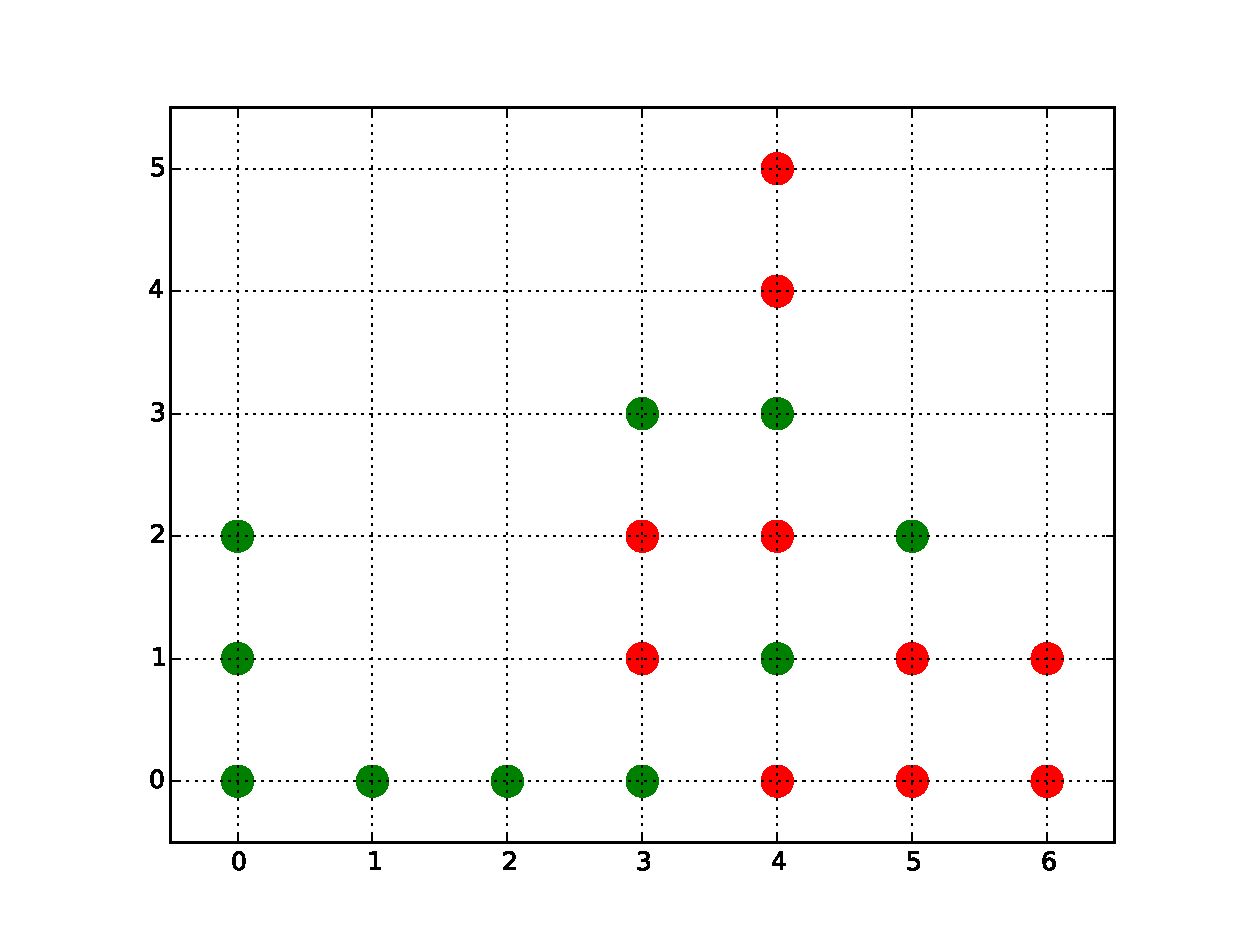
\includegraphics[scale = 0.5]{figuras/Tablero.eps}
\caption{Posición donde el jugador verde gana.}
\label{fig:tablero}
\end{figure}


\section{Algoritmo de Q-learning}

\par El algoritmo consiste en explorar la mayor cantidad de configuraciones 
posibles del juego. Durante el entrenamiento (etapa de exploración), los 
jugadores actualizan una magnitud $Q(s,a)$ que representa la ganancia o 
valorización de realizar la acción $a$ en el estado $s$. Cuando un jugador 
realiza una acción ganadora (aquella que lo conduce a un estado con cuatro 
fichas alineadas) recibe una recompensa lo que lo lleva, en el 
transcurso del entrenamiento, a valorizar positivamente las 
acciones que lo acercaron a dicho estado. 
\par Finalizado el entrenamiento, la mejor estrategia teórica consiste en, dado 
un estado $s$, elegir la acción $a$ que maximize $Q(s,a)$ (etapa de 
explotación).

\subsection{Estructura de datos}

\par Almacenamos la ganancia $Q(s,a)$ en un diccionario cuyas entradas son un 
estado representado con una variable \emph{string} de 42 caracteres de largo. 
Así por ejemplo el \emph{string} '0021000....0' representa un estado donde 
el primer jugador tiene una ficha en la cuarta columna, el segundo jugador en 
la tercera, y el resto del tablero se encuentra vacío. Inicializamos los valores de $Q(s,a)$ con un número real aleatorio entre 0 y 1.

\subsection{Representación del problema}

\par Decidimos pensar el juego como la evolución de un único sistema que puede 
encontrarse en cualquiera de los estados mencionados en la introducción. Para 
ello en lugar de distinguir entre dos jugadores observamos que para cada estado 
queda inmediatamente determinado cuál de ambos contrincantes debe mover por la 
paridad del número de fichas del mismo; así si el sistema tiene una cantidad par 
de fichas, necesariamente juega el primer jugador en alguna de las columnas 
disponibles, caso contrario lo hace el segundo.
\par Por otro lado, consideramos que una correcta actualización de la ganancia 
$Q(s,a)$ viene dada por la ecuación \ref{eq:Q}, donde $R(s,a)$ es la recompensa 
de realizar una acción $a$ en el estado $s$, $s'$ es el estado obtenido al 
realizar $a$ en $s$, y $a'$ es cualquiera de la acciones posibles en el estado 
$s'$.
\begin{equation}
Q^{n+1}(s,a) = Q^{n}(s,a) + \alpha (R(s,a) - \gamma (max_{a'}Q^n(s',a') - Q^n(s,a))
\label{eq:Q}
\end{equation} 
Dado un estado, la valorización de una acción:
\begin{itemize}
\item aumenta si al realizar una acción, de esta se obtiene una recompensa (en este caso se gana el juego)
\item disminuye si la mejor acción del siguiente estado (que corresponde al otro jugador) está muy valorizada. Es decir cada jugador trata de tomar acciones que no lleven a un estado donde el otro jugador tenga una muy buena jugada.
\end{itemize}
Pensándolo de esta manera, en el algoritmo solo se introducen recompensas 
positivas. Cuando un jugador gane y reciba una recompensa, el otro jugador 
desvaluará la acción que llevó al sistema a ese estado, y valorará más las 
otras. Utilizamos $\alpha = 0.01$, $\gamma = 0.9$, y una recompensa $R = 100$.

\subsection{Exploración de los estados: temperatura}

\par Durante la fase de entrenamiento no existe \emph{a priori} ninguna 
restricción sobre las acciones que el sistema decida explorar; estas pueden ser 
escogidas totalmente al azar. Siguiendo esta estrategia, y al cabo de 
cierto tiempo, la exploración recorrerá múltiples veces todos los pares 
$(s,a)$ logrando una valorización adecuada de todas las acciones posibles para 
todos los estados. Sin embargo dada la ingente cantidad de estados posibles 
mencionada en la introducción, aun en un tablero pequeño esta estrategia 
resulta impracticable en un tiempo razonable. Resulta entonces útil introducir 
una magnitud (temperatura) que permita focalizar la búsqueda en aquellas ramas 
del árbol de jugadas que, a la luz del entrenamiento transcurrido, parezcan la 
más promisorias. Cuando la temperatura sea máxima el sistema elegirá en forma 
equiprobable entre las acciones posibles (exploración pura), mientras que 
cuando sea mínima escogerá aquella acción que maximize $Q$ (explotación pura).
\par En suma, la disminución progresiva de este parámetro nos permite variar la 
estrategia de entrenamiento desde una puramente exploratoria y abarcativa hacia 
otra focalizada sobre las ramas más promisorias del árbol de jugadas.

\subsection{Modificaciones agregadas}

\par Suponiendo que el algoritmo no iba a converger, generamos una versión alternatica ``con visión''. En la misma los jugadores, a temperatura nula, no dejan pasar la oportunidad de generar un 4 en línea ante la presencia de tres fichas alineadas e intentan evitar, ante una situación en que su oponente se encuentre con tres fichas alineadas, que este logre conectar una cuarta.
\par En un contexto donde los jugadores tienen este tipo de visi\'on, la \'unica forma de ganar es que aprendan a armar las "trampas" en las que el oponente no puede bloquear, es decir, donde hay dos posibles 4 en línea.

\section{Resultados}

\par Tras entrenar el algoritmo durante tres días, obtuvimos una valuación de $Q$ con la cual corrimos una competencia entre los jugadores, donde el jugador 2 basó su juego en dichos valores, mientras que el jugador 1 tomó acciones aleatorias, obteniendo los siguientes resultados:

\begin{figure}[H]
    \centering
    \begin{subfigure}[b]{0.45\textwidth}
      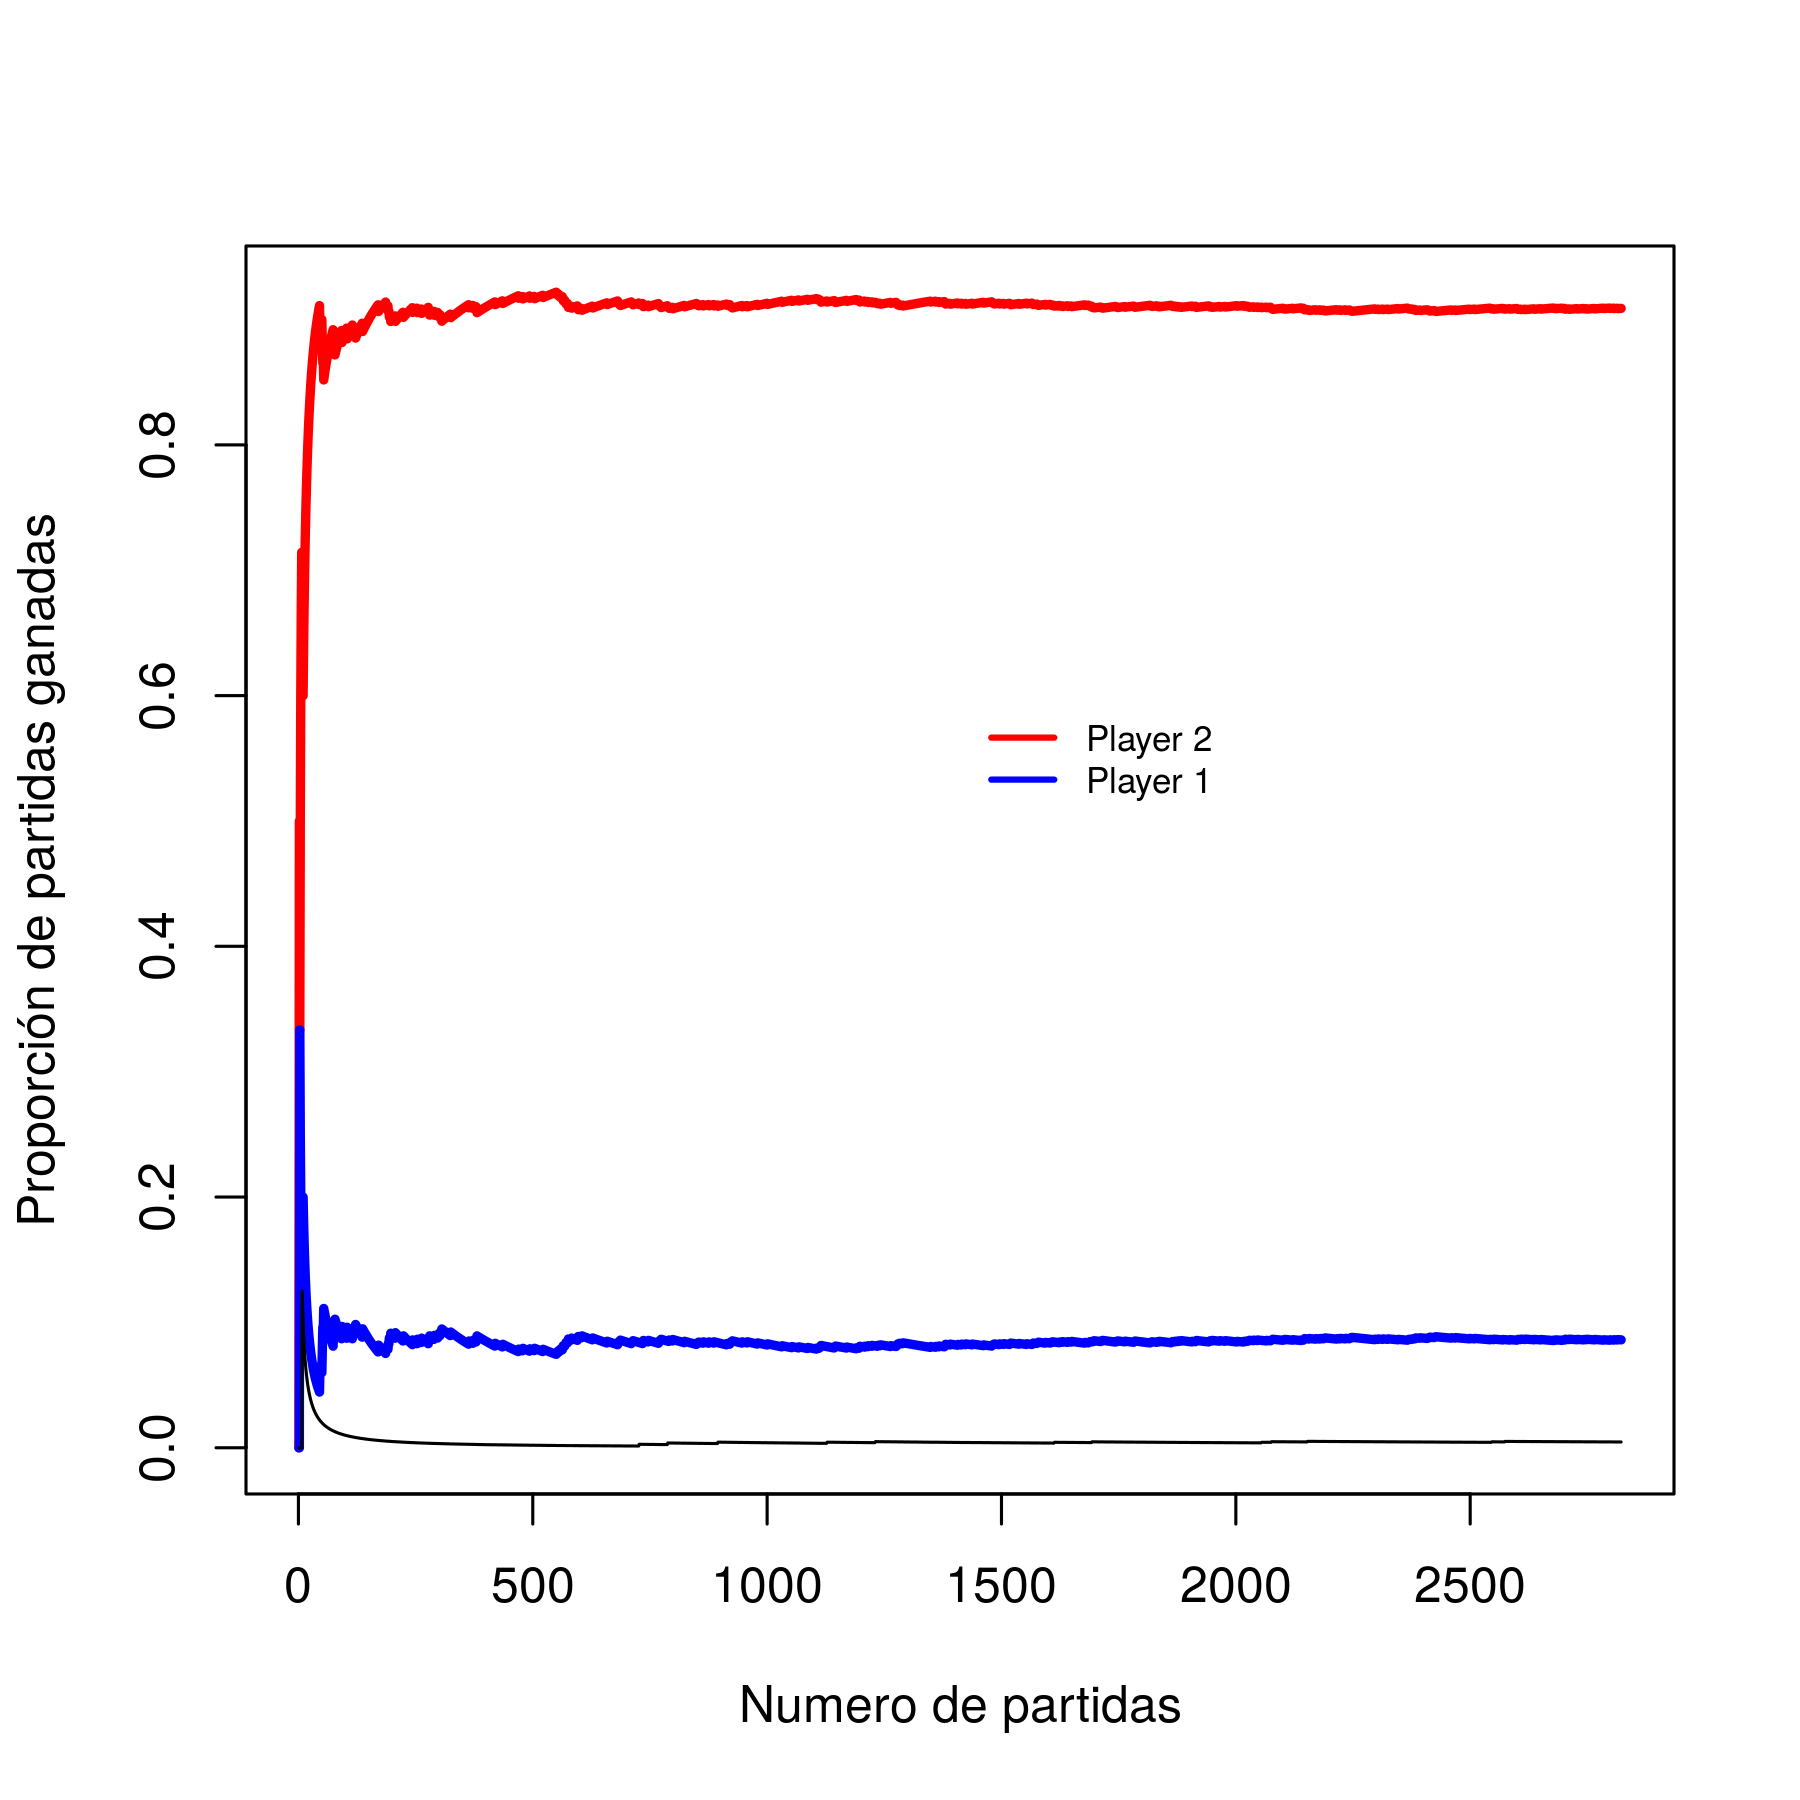
\includegraphics[width=\textwidth]{Imagenes/SinVision_luchaNoLibre_QsinVison_reverse}
    \end{subfigure}
    \caption{Jugador 1 al azar. Jugador 2 basado en los valores Q}
\end{figure}

\par En este experimento, dejamos la ``temperatura''(GUS FIJATE QUE QUISISTE PONER ACA). 
Ahora hacemos un experimiento similar, pero variando la temperatura de un solo jugador y dejando el otro jugando completamente al azar. Hacemos esto para los dos jugadores. Lo que obtenemos es lo siguiente: 

\begin{figure}[H]
    \centering
    \begin{subfigure}[b]{0.45\textwidth}
      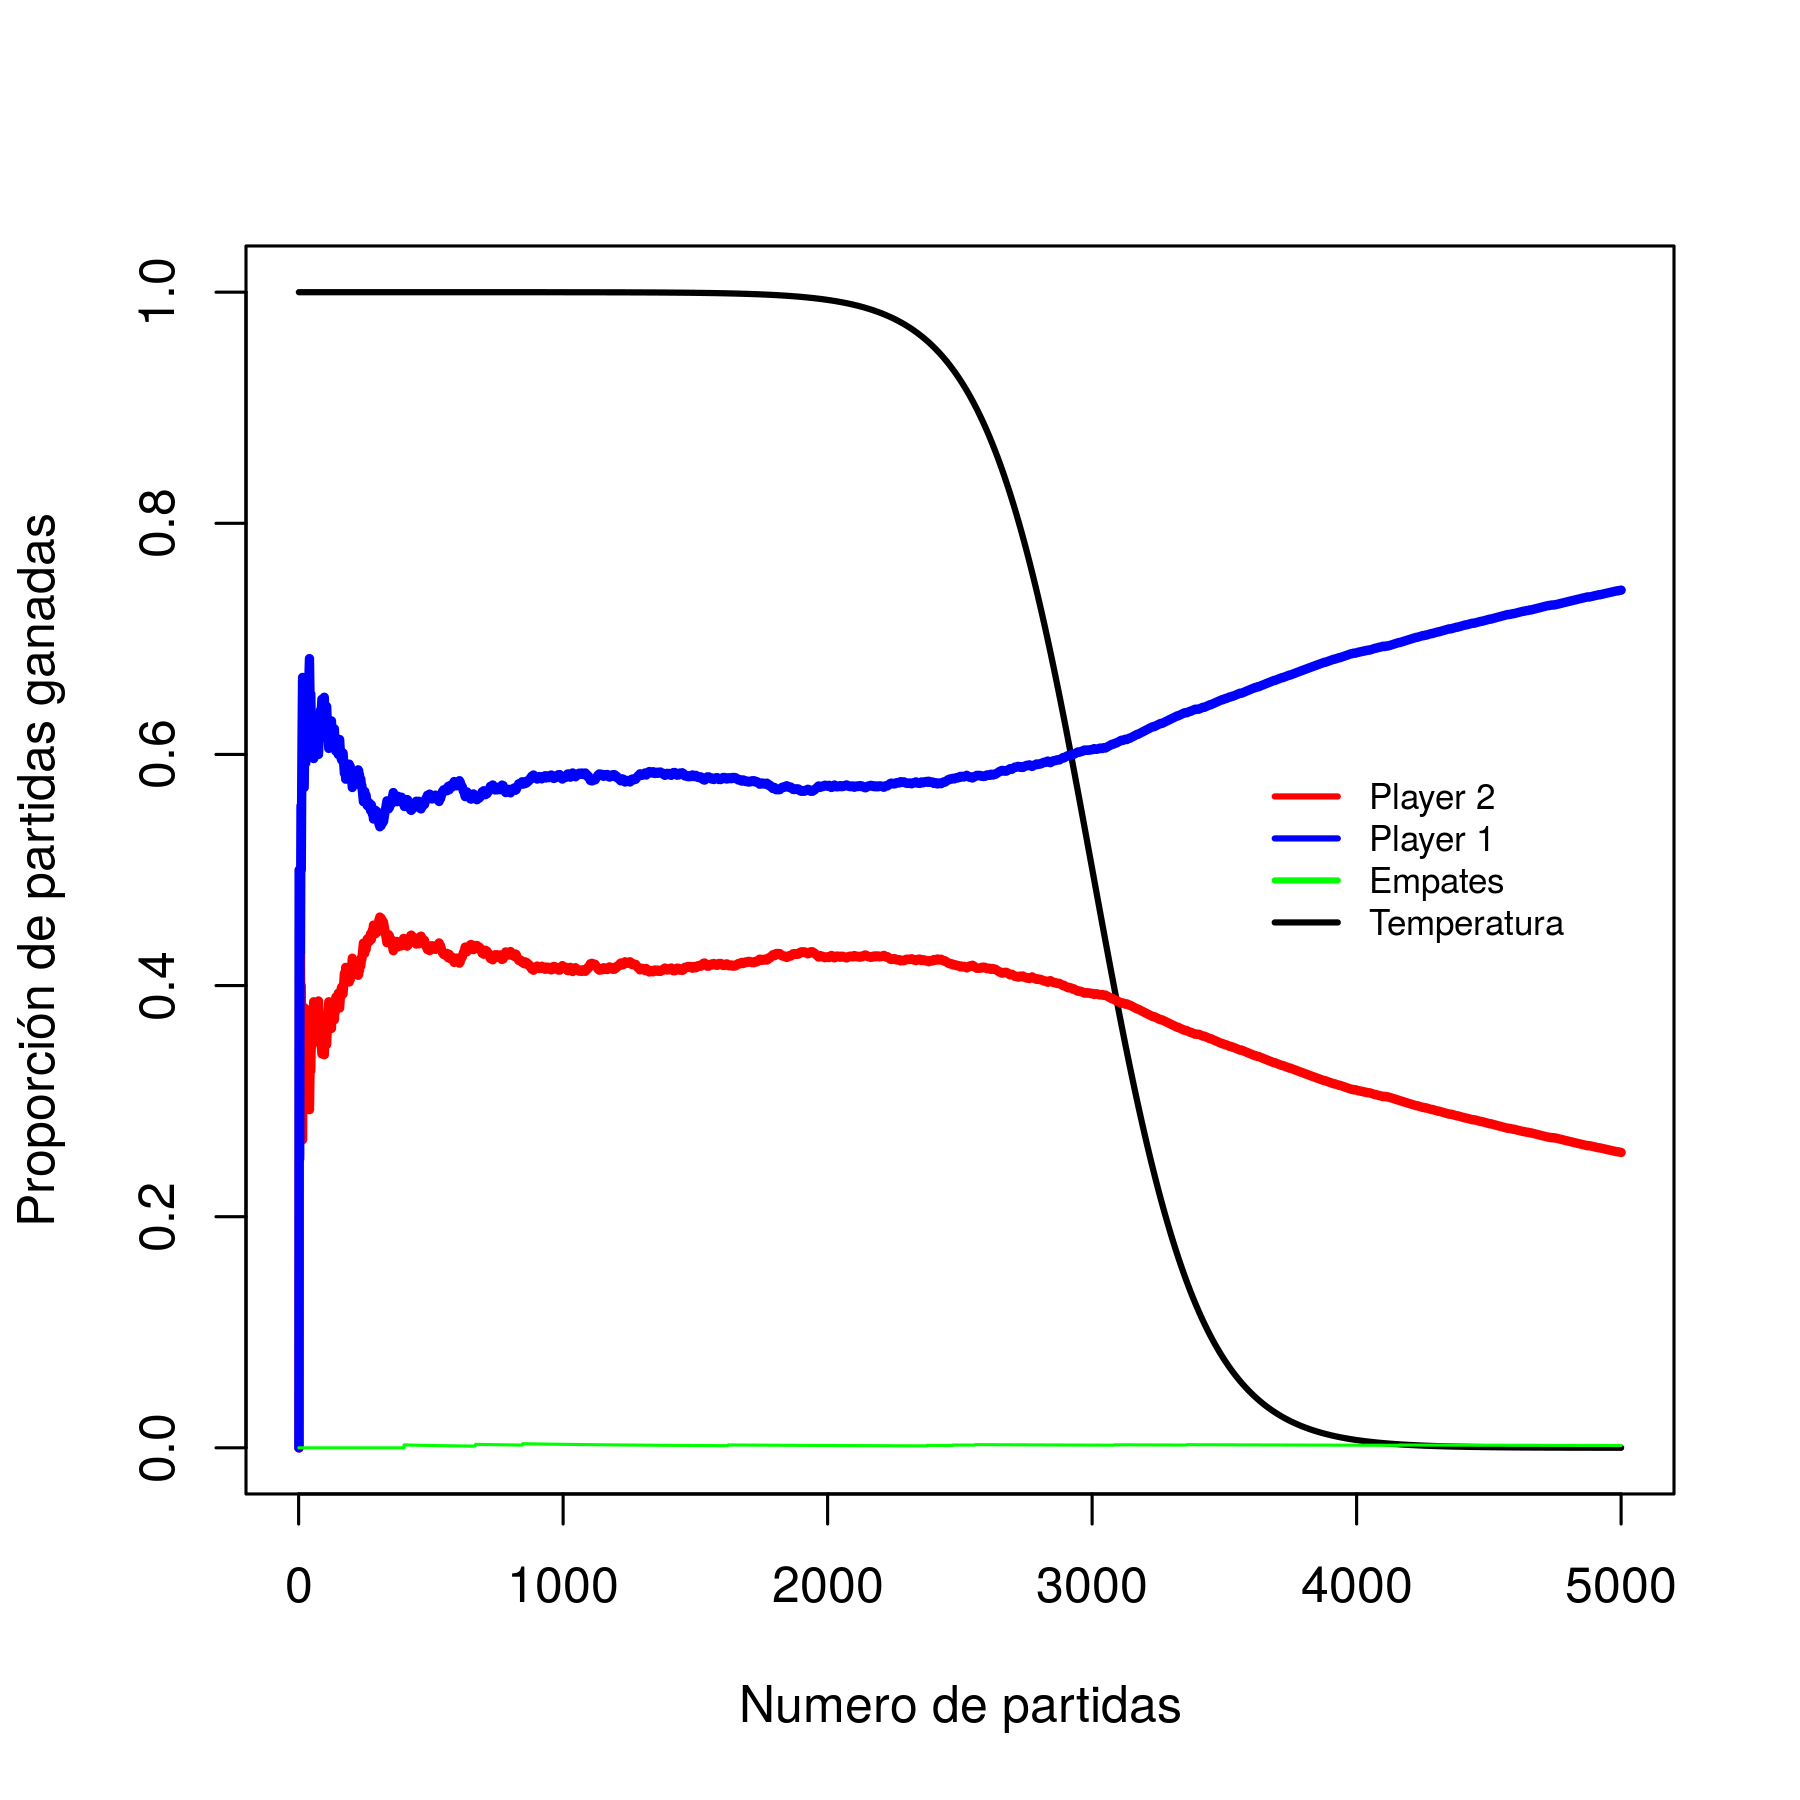
\includegraphics[width=\textwidth]{Imagenes/SinVision_disipacion_QsinVison}
    \end{subfigure}
    \begin{subfigure}[b]{0.45\textwidth}
      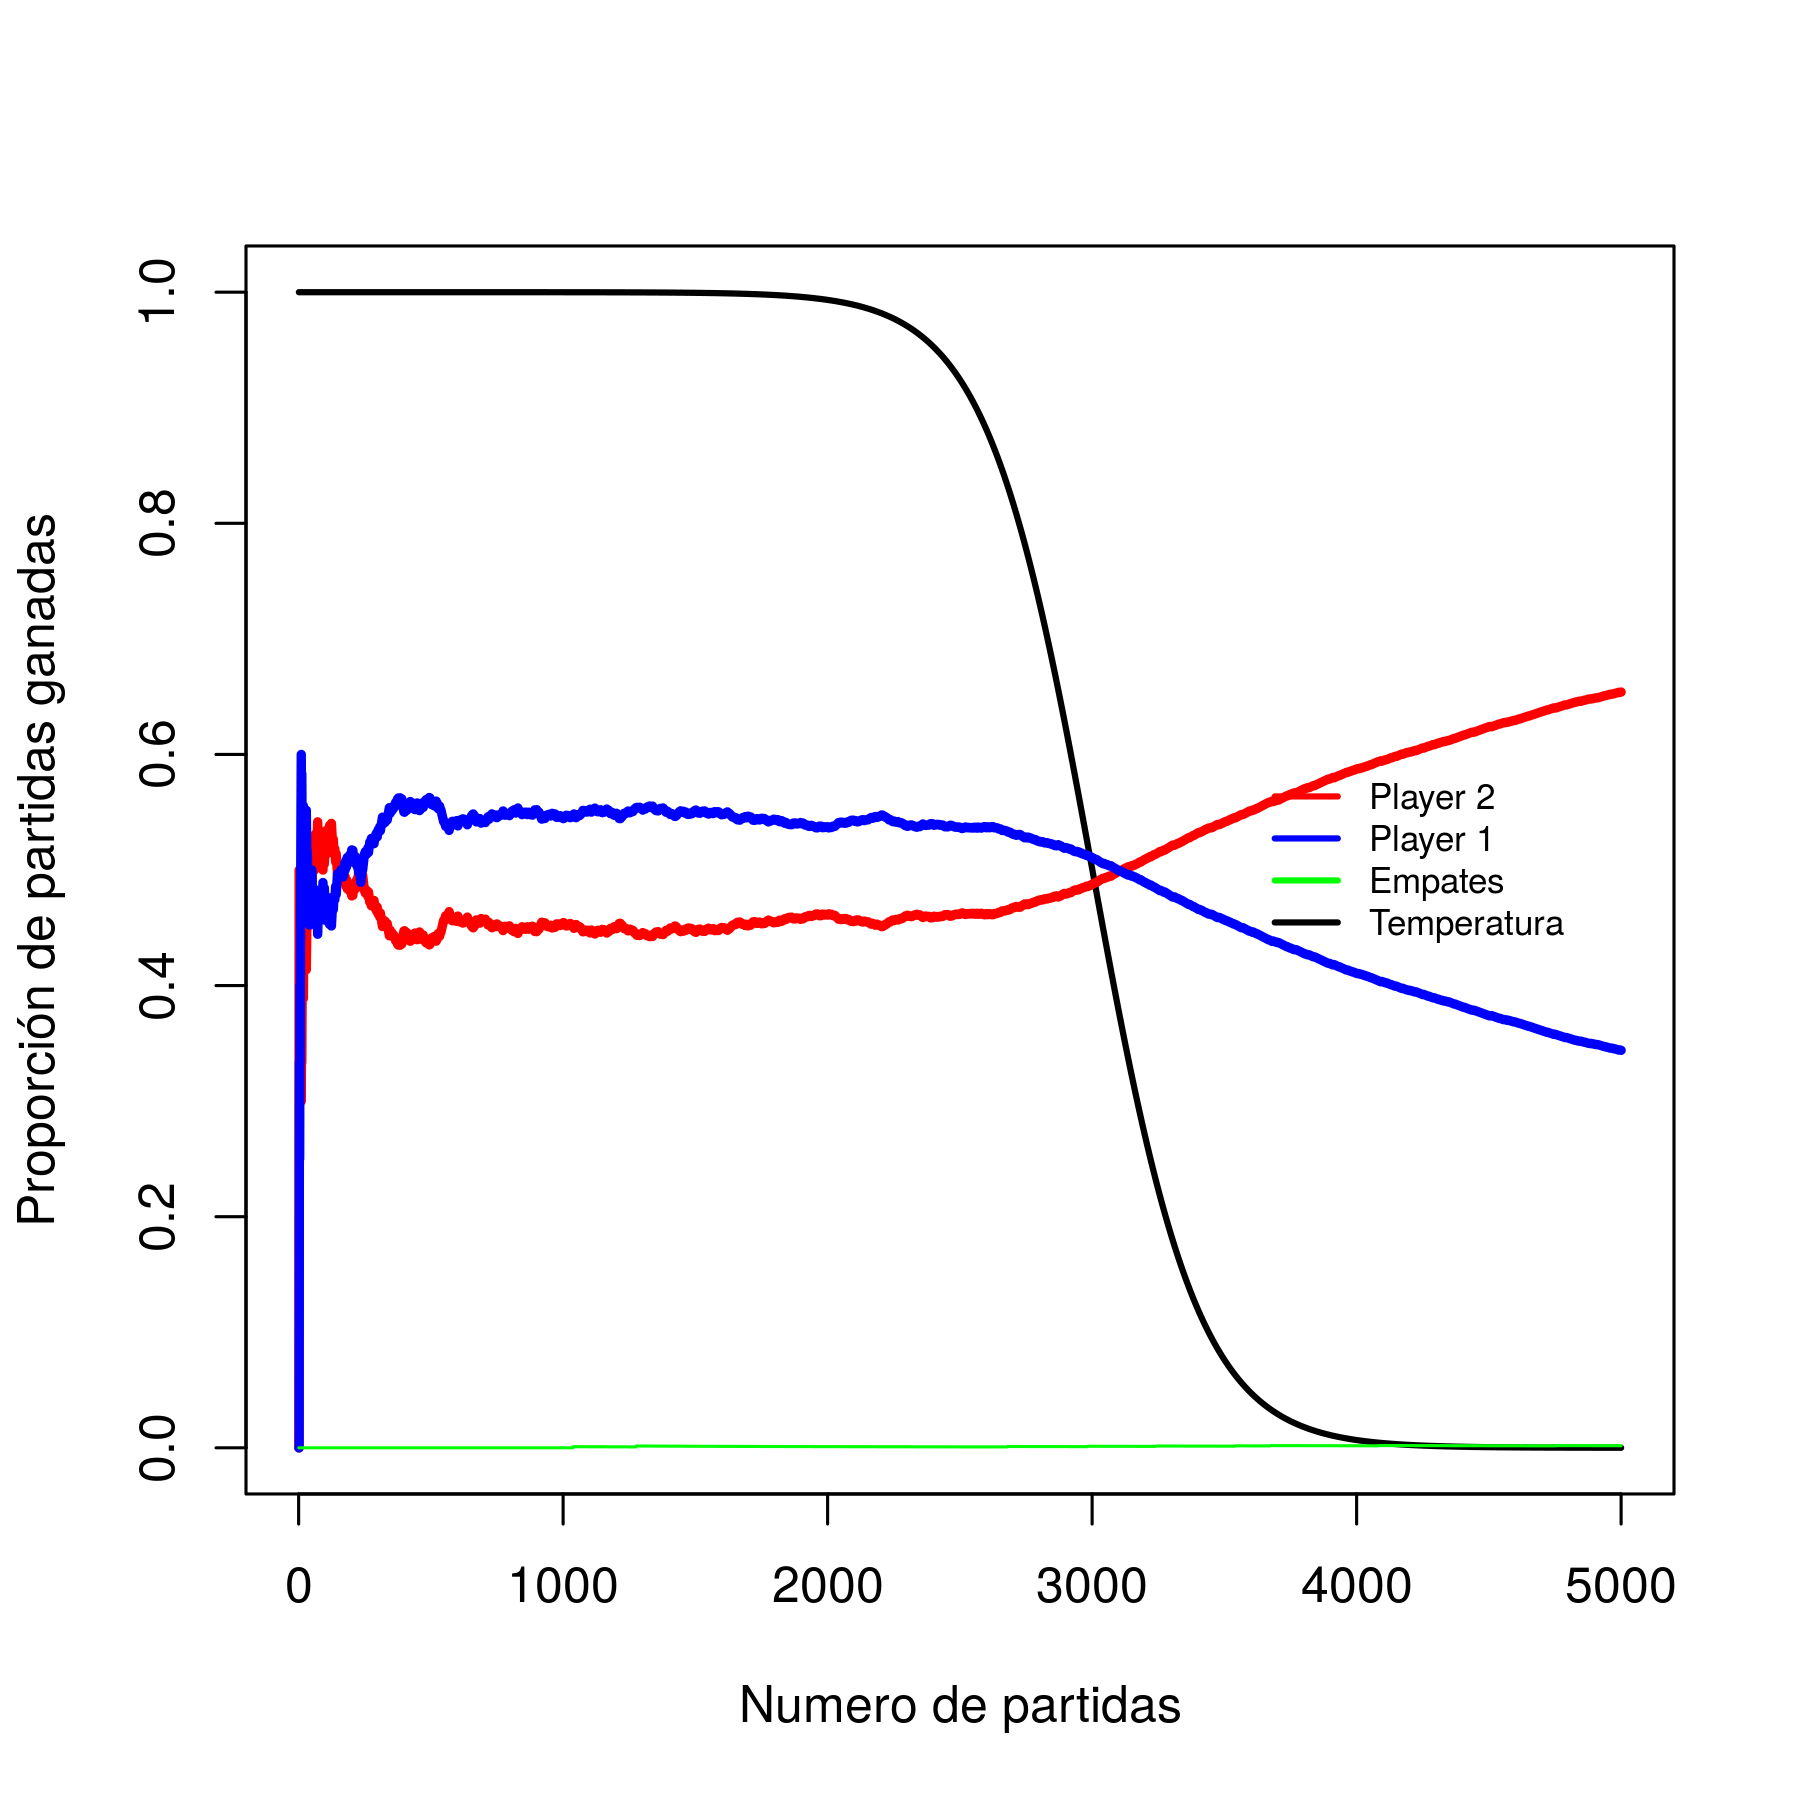
\includegraphics[width=\textwidth]{Imagenes/SinVision_disipacion_QsinVison_reverse}
    \end{subfigure}
    \caption{Un jugador al azar y un jugador bajando la temperatura}
\end{figure}

\par La versión modificada de actualización de Q ``con visión'' también aprendió. Esta versión la dejamos corriendo del sábado a la mañana hasta el domingo a las 23.59hs. Usando el Q resultante corrimos una competencia de los jugadores, ahora sin visión, basados solo en el Q. En el experimiento en el que se varía la temperatura de un jugador, mientras que el otro juega al azar, los resultados son los siguientes:

\begin{figure}[H]
    \centering
    \begin{subfigure}[b]{0.45\textwidth}
      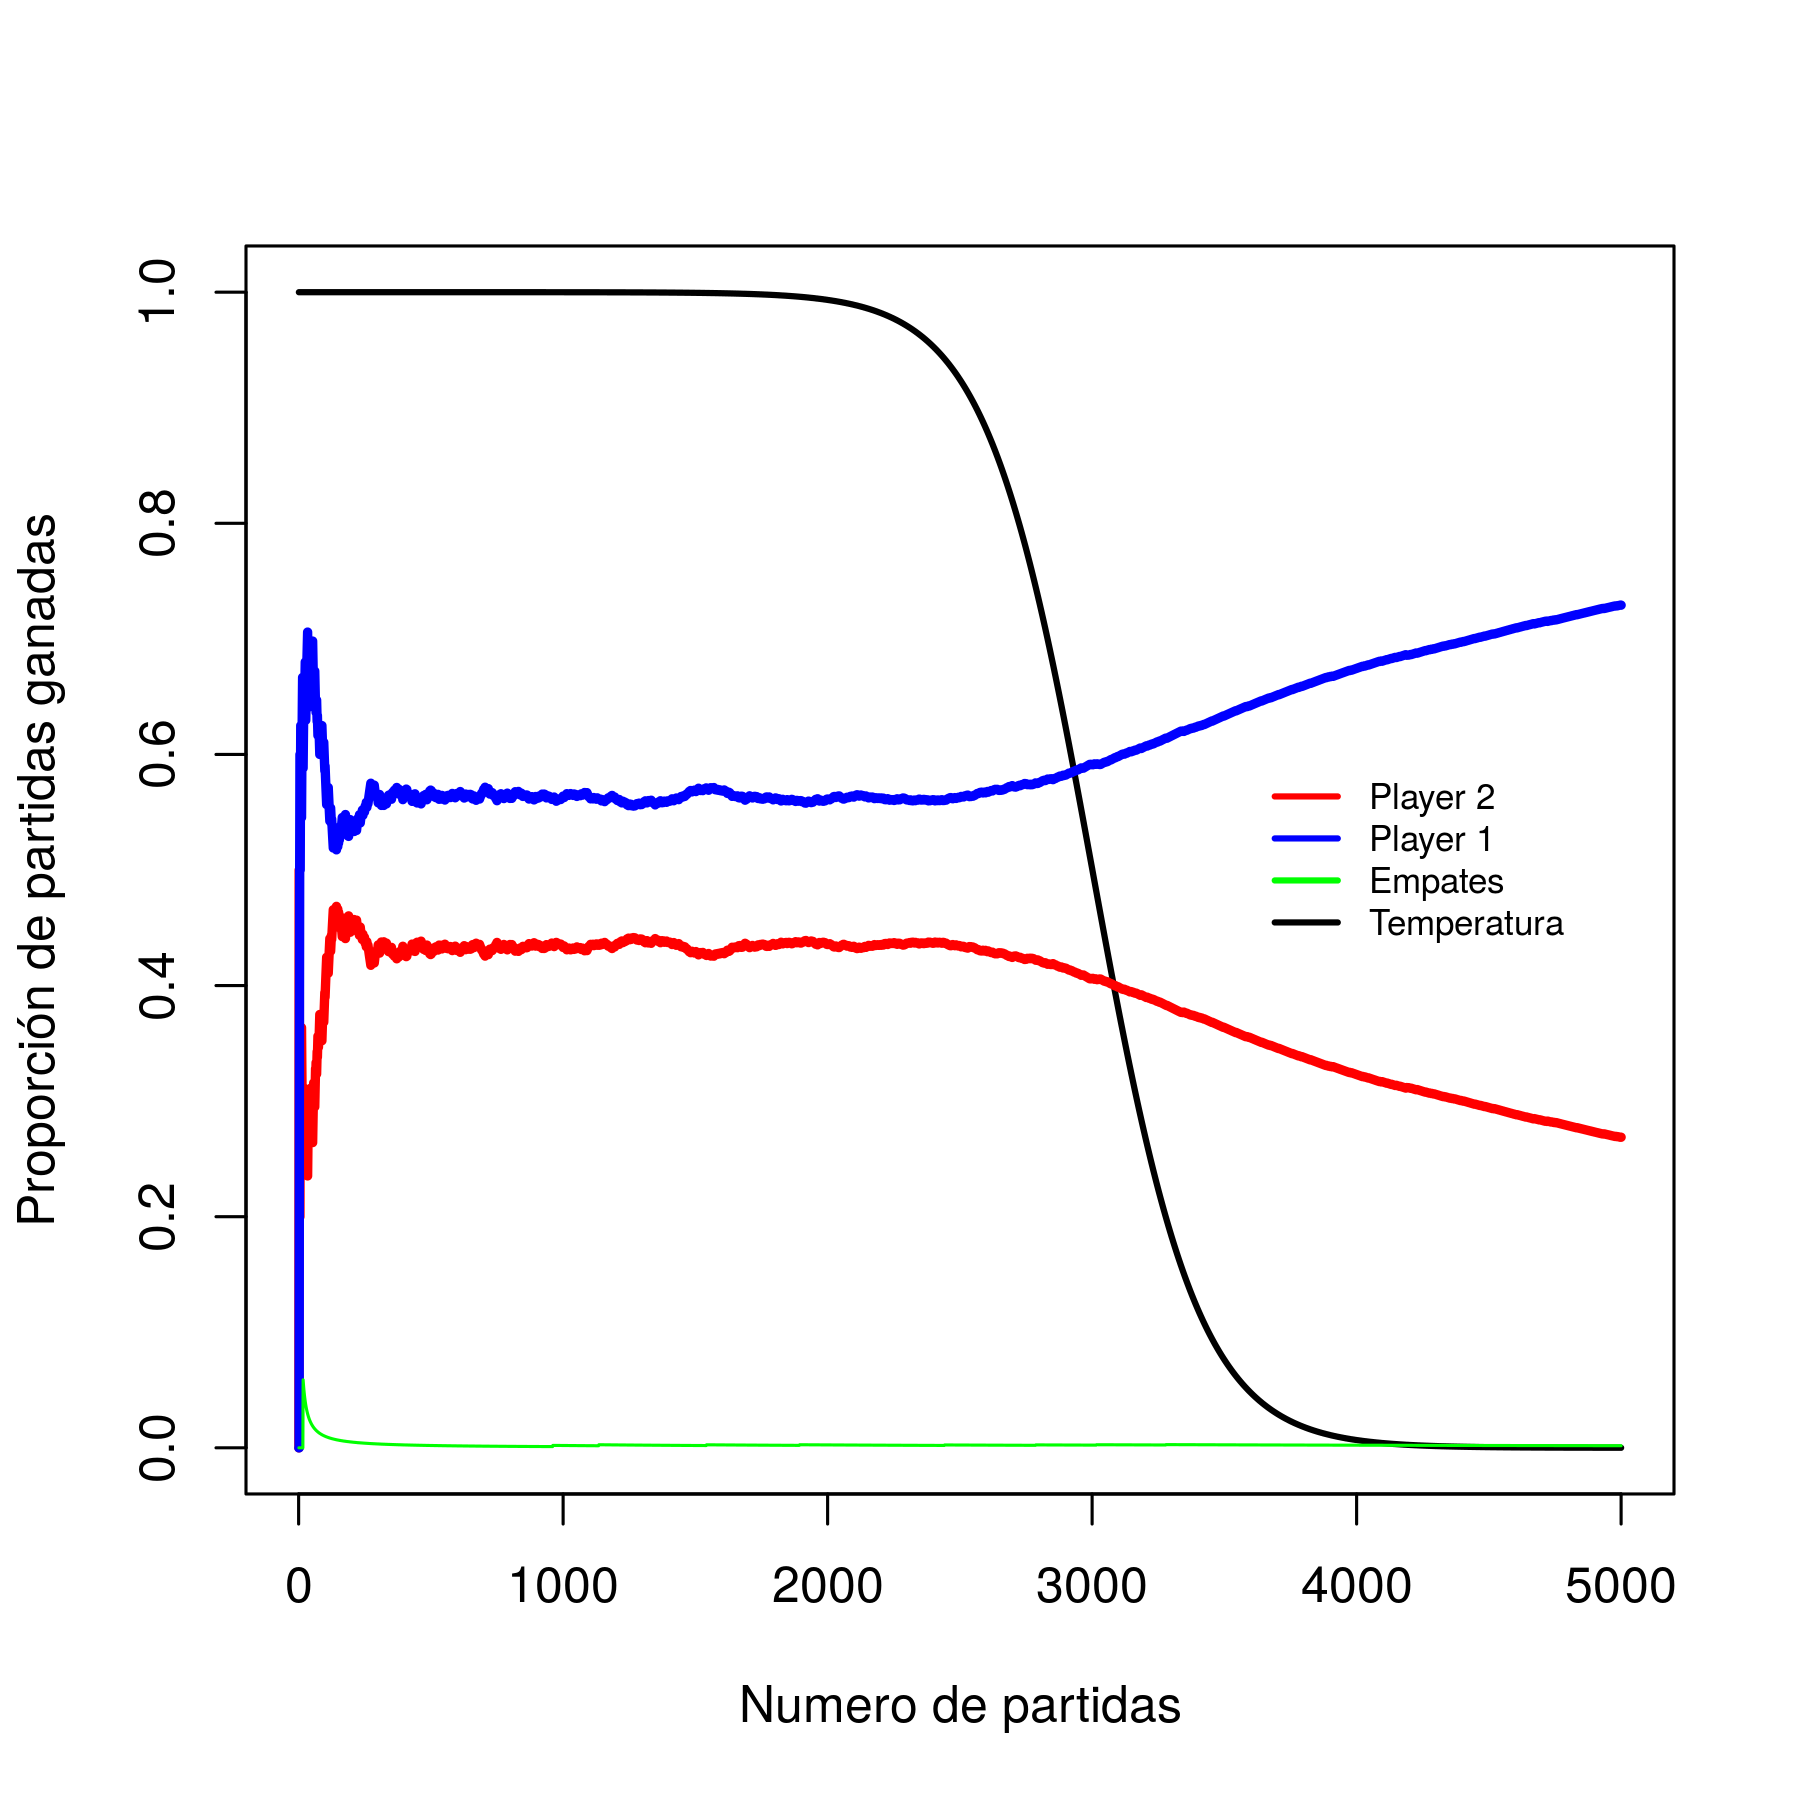
\includegraphics[width=\textwidth]{Imagenes/SinVision_disipacion_QconVison}
    \end{subfigure}
\end{figure}


\section{Estrategias exploradas}
\par Utilizando el algoritmo presentado en la ecuación \ref{eq:Q} exploramos 
el impacto de la estrategia adoptada sobre el desempeño de juego. Convenimos en 
entrenar siempre al jugador 2 y medir su desempeño al enfrentarse con un 
contendiente (jugador 1) que elije siempre acciones al azar (temperatura 
infinita). Para anular cualquier posible impacto de la iniciativa sobre el 
desempeño definimos de manera equiprobable qué jugador mueve primero en cada 
partido, así en promedio ambos jugadores comenzarán la misma cantidad de veces.

\subsection{E-greedy}
\par Una de las estregias de aprendizaje que estudiamos fue la \emph{e-greedy} 
en la cual el jugador número 2 elije con probabilidad $\epsilon$ una acción al 
azar y con probabilidad $1-\epsilon$ la acción con la mayor valorización. Se 
trata de una estrategia que combina exploración y explotación en proporción 
constante. Profundizamos para los siguientes valores de $\epsilon = 
0.1$, $0.5$, $1.00$, y $0.00$. Las dos últimas se corresponden, respectivamente, 
con los casos puramente exploratorio y puramente explotatorio. En la figura 
\ref{fig:e_greedy} observamos la evolución de las victorias acumuladas de cada 
jugador en función del número de jugadas.
\par De la figura \ref{fig:e_greedy} concluímos que un valor bajo $\epsilon$, 
pero no nulo, ayuda al jugador 2 a sacar cierta ventaja del 1. En este caso, el 
jugador explora el 10\% de las veces y el resto juega a la mejor jugada. 
Observamos que a partir del paso $10000$, la exploración inicial ya es 
suficiente, y comienza a sacar ventaja de la información ganada durante ese 
lapso. Cabe mencionar que solo entrenamos durante $100000$ partidas, lo que da lugar a un número de estados visitados que podemos acotar superiomente por $42$ x$100000$, que es del orden de la millonésima parte del total de estados, mencionados en la introducción.

\begin{figure}
\centering
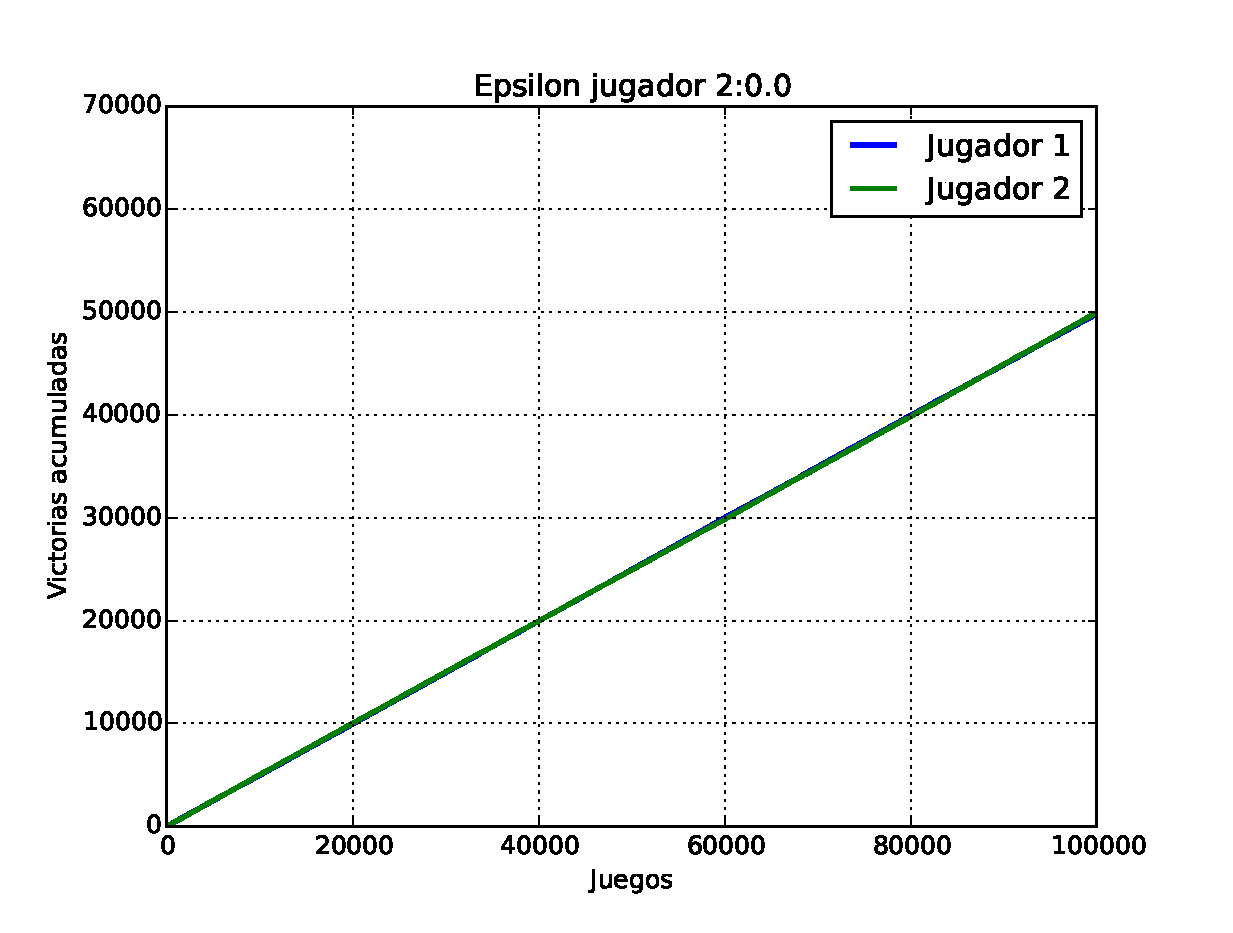
\includegraphics[scale = 0.3]{figuras/Epsilon00.eps}
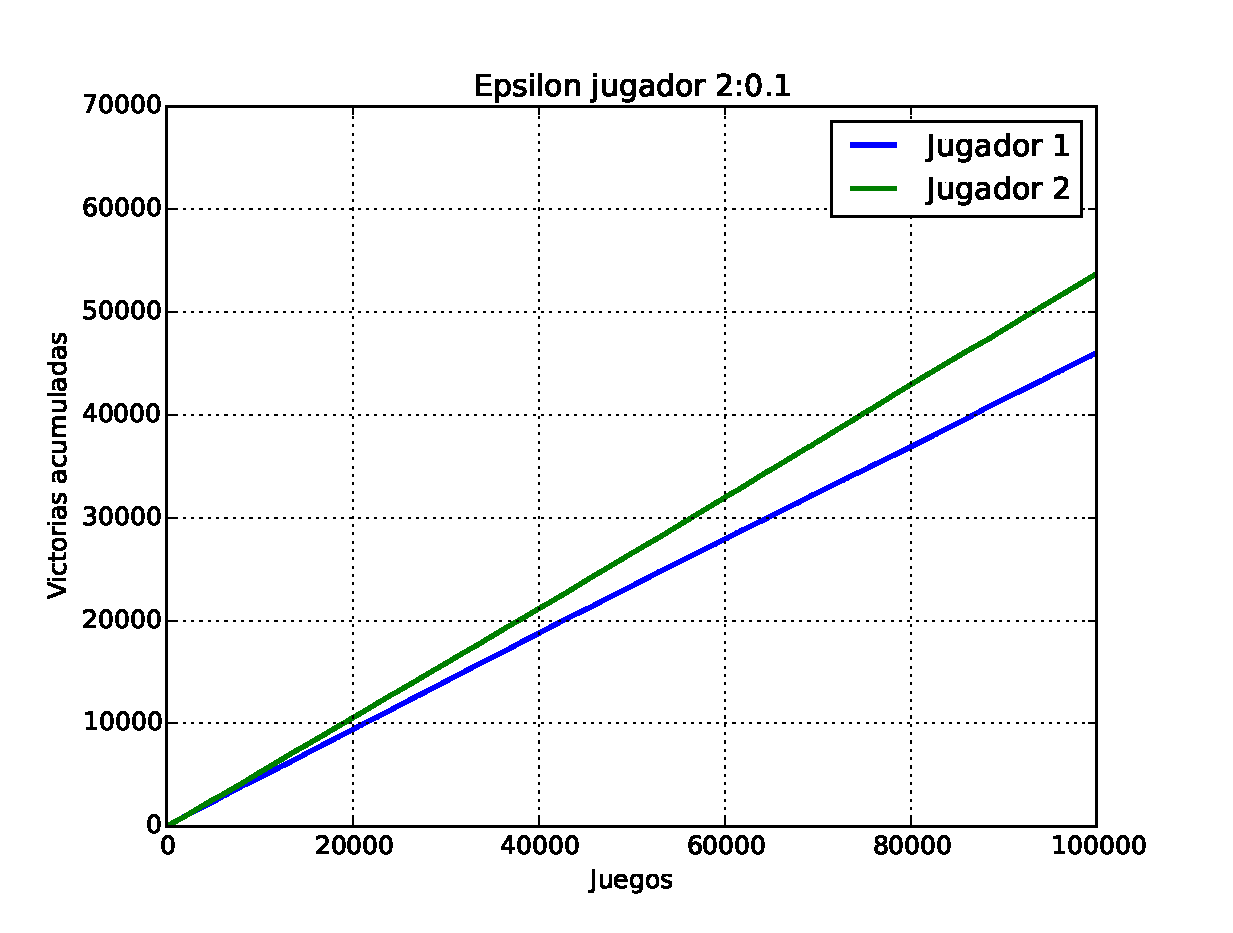
\includegraphics[scale = 0.3]{figuras/Epsilon01.eps}\\
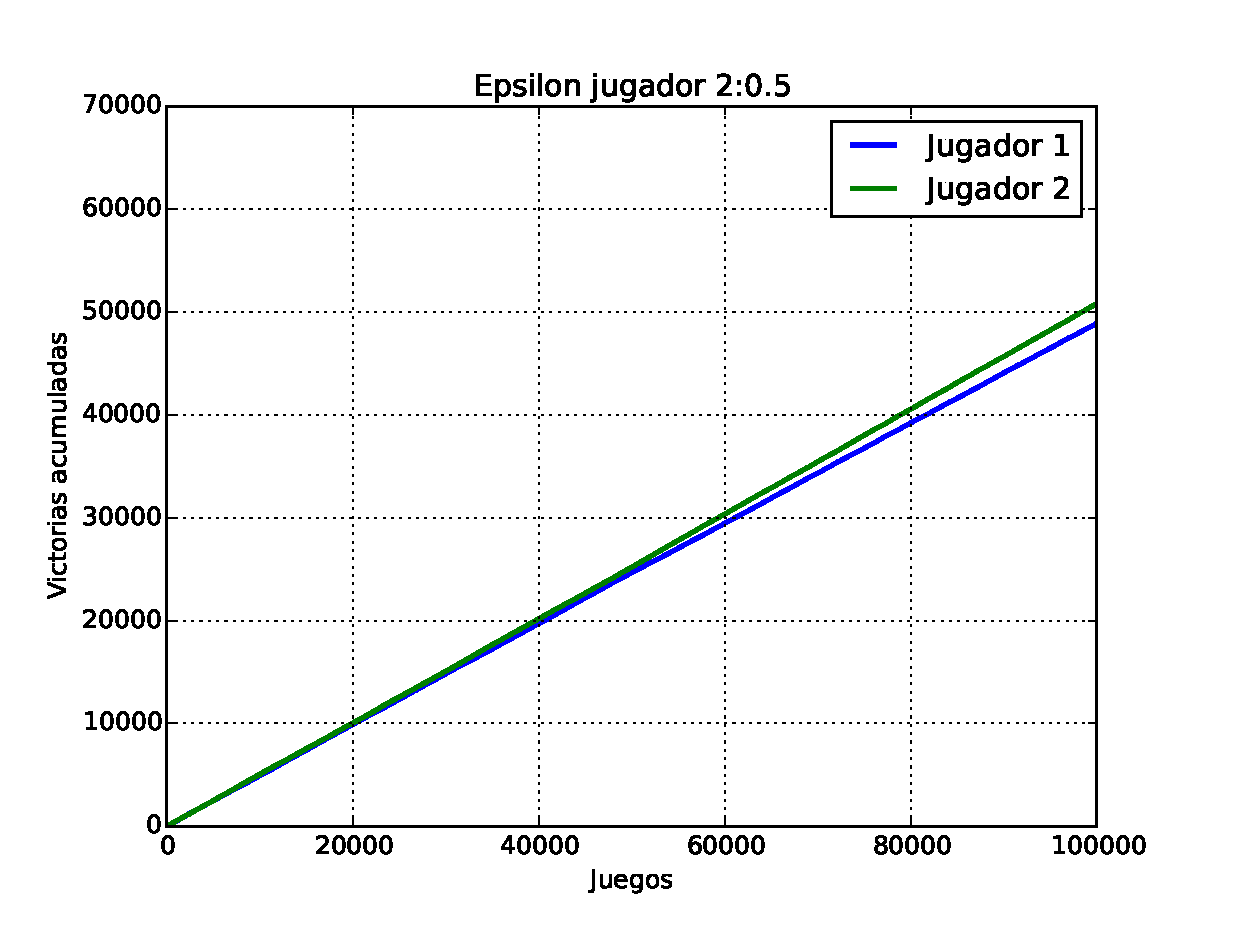
\includegraphics[scale = 0.3]{figuras/Epsilon05.eps}
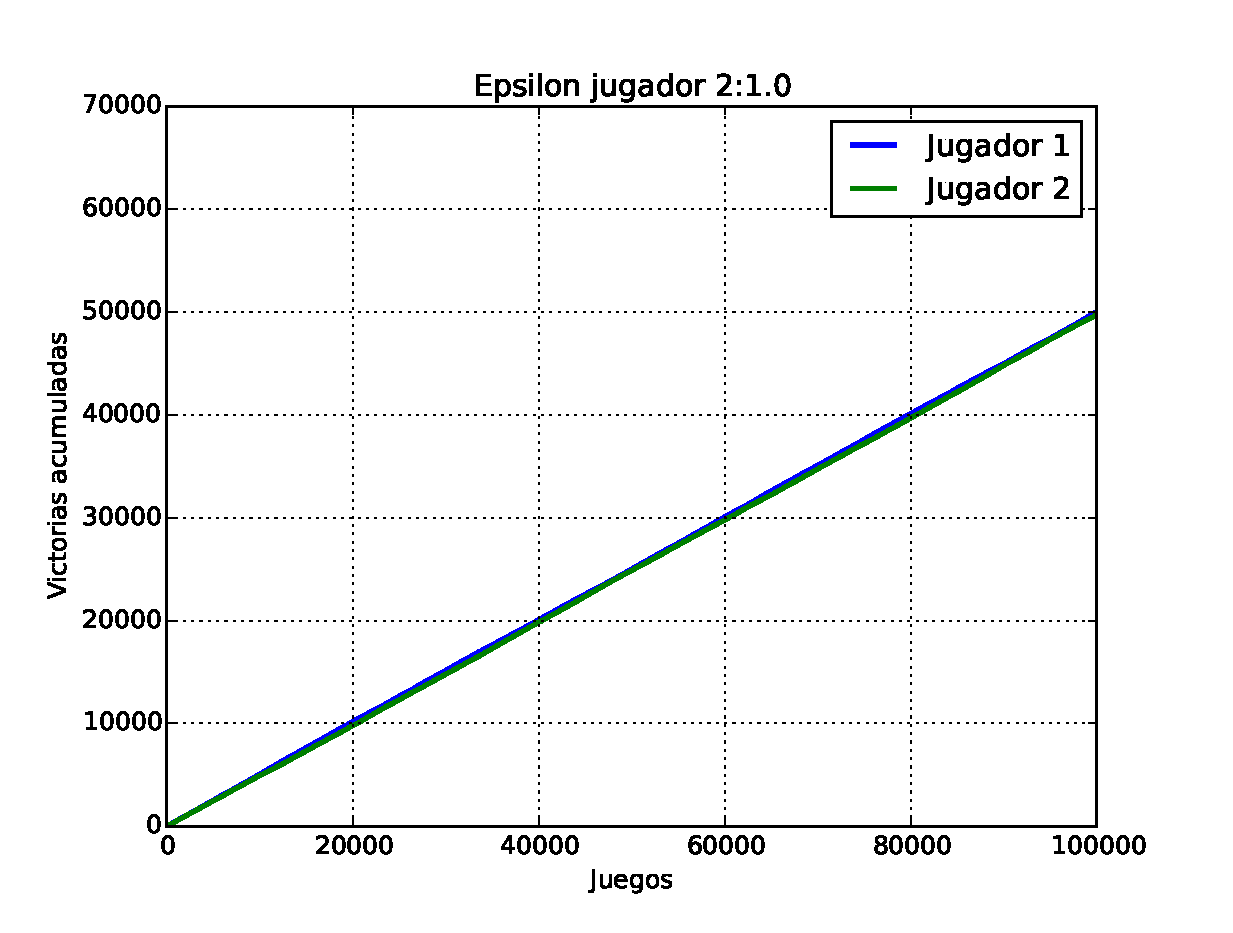
\includegraphics[scale = 0.3]{figuras/Epsilon10.eps}
\caption{Victorias acumuladas en función del número de juegos realizados. Se 
observa que el jugador 2 saca ventaja al implementar una estrategia 
\emph{e-greedy} con $\epsilon$ bajos. De izquierda a derecha, y de arriba hacia 
abajo, $\epsilon = $ $0.00$, $0.10$, $0.50$ y $1.00$.}
\label{fig:e_greedy}
\end{figure}

\subsection{Softmax}
\par Otra estrategia que exploramos fue \emph{Softmax}, en la cual la acción es 
escogida con una probabilidad dada por la ecuación \ref{eq:softmax}, donde 
$T$ es la temperatura del sistema. La idea original fue la implementación de 
una temperatura inicial alta que disminuimos gradualmente con el número de 
partidos disputados, de esta forma el jugador se centrará al comienzo en la 
exploración pero a medida de que la temperatura descienda variará hacia una 
mayor explotación. Sin embargo observamos que los valores $Q$ no estaban 
acotados ni superior ni inferiormente por lo que los cálculos de la 
exponencial arrojaron errores númericos insalvables. Nos resultó 
muy dificil explorar este algoritmo.
\begin{equation}
P(s,a) = \frac{\exp(Q(s,a)/T)}{\sum_{a'}{\exp(Q(s,a')/T)}}
\label{eq:softmax}
\end{equation}

\section{Conclusiones}

\par Implementamos un algoritmo basado en Q-learning para entrenar jugadores virtuales del juego 4 en línea. El algoritmo basicamente consistió en explorar con diferentes estrategias, la mayor cantidad de estados posibles del juego y valorizar la acciones que se toman en cada uno de ellos.
\par Observamos el comportamiento de un jugador que toma decisiones con una dada estrategia en contra de uno que toma acciones aleatoriamente. En particular, empleamos la estrategia \emph{e-greedy}, donde observamos que el jugador entrenado saca una leve ventaja para valores de $\epsilon$ pequeños pero no nulos, es decir, en escenarios donde la exploración aleatoria es poco frecuente. Para otras estrategias, nos enfrentamos a problemas númericos que no nos permitieron avanzarcon la investigación.
\par Por otro lado, exploramos una versión alternativa que llamamos ``con visión''. (ACA GUS ESCRIBI LO QUE QUIERAS)


\end{document}
